% use pdfpc to present
\documentclass[]{beamer}

\usepackage{color}
\usepackage{pgfpages}
\usepackage{url}
\usepackage{hyperref}

\setbeameroption{show notes on second screen=right}

%TODO: Add Images

%document specific info
\title{Physical Security}
\subtitle{or ``Why is that man in my server room''}
\author{Stephen ``ToxicSauce'' Walker-Weinshenker}
\institute{
  \inst{}
  Department of Computer Science\\
  Colorado State University
  \and
  \inst{}
  Department of Electrical and Computer Engineering\\
  Colorado State University
}
\date{\today}
\subject{subject}

%beamer template
\definecolor{HDred}{RGB}{171,31,36}
\setbeamercolor{background canvas}{bg=gray}
\setbeamercolor{title}{fg=HDred}
\setbeamercolor{frametitle}{fg=HDred}
\setbeamercolor{logo}{bg=gray}

\logo{
\includegraphics[height=1.5cm]{logo.png}}

\useoutertheme[hideallsubsections]{sidebar}


\begin{document}
\frame{\titlepage}

% \begin{frame}
% \frametitle{Table of Contents}
% \tableofcontents%[current section]
% \end{frame}

\begin{frame}
  \frametitle{What is Physical Security}
\begin{itemize}
  \item Controlling physical access to something
  \item Normally used in the context of a building or room
\end{itemize}
\begin{alertblock}{Note:}
  Any type of Security is a balance between security, and convience of access
\end{alertblock}
\note[item]{there is no perfect security}
\end{frame}

\begin{frame}
  \frametitle{Primary Elements of Physical Security}
\begin{itemize}
  \item Physical Structure of Building and Site
  \begin{itemize}
    \item Doors
    \item Windows
    \item Walls
    \item Roofs
    \item Floors
    \item Perimeter of Property
  \end{itemize}
\end{itemize}

\end{frame}



\begin{frame}
  \frametitle{Primary Elements of Physical Security}
\begin{itemize}
  \item Secure Elements of Building
  \begin{itemize}
    \item Locks and Keys
    \item Other Access Control
    \item Man Traps
    \item Vehicle Gates
  \end{itemize}
\end{itemize}

\end{frame}

\begin{frame}
  \frametitle{Human Factors}
\begin{itemize}
  \item Security Guards
  \item Other Employees

\end{itemize}
\end{frame}

\begin{frame}
  \frametitle{Security Guards}
  \begin{columns}[c]
    \column{0.5\textwidth}
    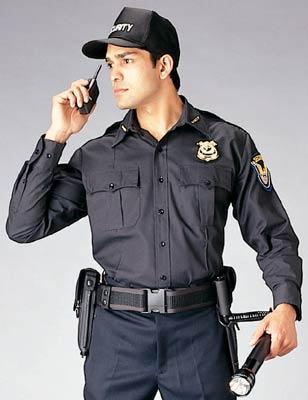
\includegraphics[width=.8\textwidth]{Security-Guard}
    \column{0.5\textwidth}

  \end{columns}
\note[item]{is there a way around the guards}
\note[item]{how attentive are they}
\note[item]{are they getting distracted}

\end{frame}



\begin{frame}
  \frametitle{Other Employees}
  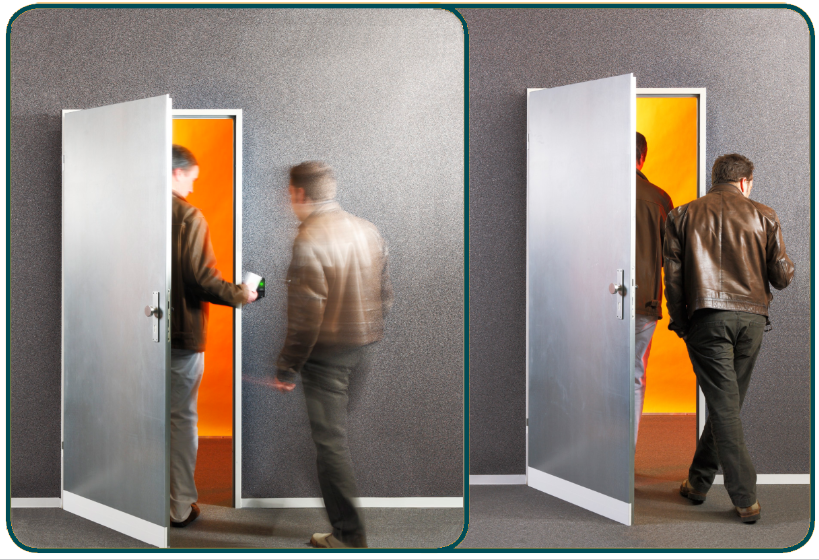
\includegraphics[width=.9\textwidth]{tailgating}
  \note[item]{tailgating}
  \note[item]{social engineering}
  \note[item]{bribery}
\end{frame}

\begin{frame}
  \frametitle{doors}
  \begin{columns}[c]
    \column{0.5\textwidth}
  \begin{itemize}
    \item frame gap
    \item REX sensor
    \item lock --- fail safe or deadly
    \item hinges
    \item door fit
  \end{itemize}
  \column{0.5\textwidth}
  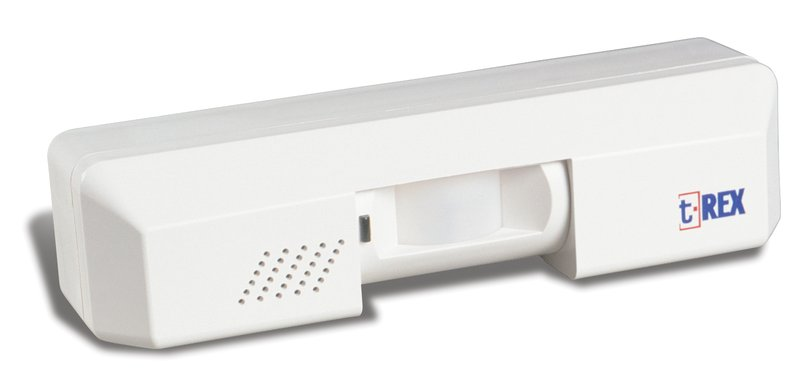
\includegraphics{T-REX}
\end{columns}
\note[item]{\url{https://www.youtube.com/watch?v=SDl4AO4ancI}}
\end{frame}

\begin{frame}
  \frametitle{Windows}
\end{frame}

\begin{frame}
  \frametitle{Walls}
\end{frame}

\begin{frame}
  \frametitle{Roofs}
\end{frame}

\begin{frame}
  \frametitle{Floors}
\end{frame}

\begin{frame}
  \frametitle{Perimeter of Property}
  \begin{itemize}
    \item vehicle gates
  \end{itemize}
\end{frame}

\begin{frame}
  \frametitle{Locks and Keys}
  \begin{itemize}
    \item most locks are shit
    \item almost all padlocks are shit
    \item good locks are not infaliable
    \item master keys/recorable locks
    \item keyboxen --- knox boxen
  \end{itemize}
\end{frame}

\begin{frame}
  \frametitle{Other Access Control}
\end{frame}

\begin{frame}
  \frametitle{Man Traps}
\end{frame}

\begin{frame}
  \frametitle{References}
  \begin{itemize}
    \item \url{http://www.securityguardpedia.com/wp-content/uploads/2015/02/Security-Guard-East-Region.jpg}
    \item \url{http://kudos-security.com/wp-content/uploads/2015/06/TAILGATING.png}
    \item \url{http://cms.dsc.com/media/products/lthumbs/i_T-REX.jpg}
    \item \url{https://www.youtube.com/watch?v=4YYvBLAF4T8}
  \end{itemize}

\end{frame}

\end{document}
